\documentclass[12pt]{article}

\usepackage[utf8]{inputenc}					% pacote para acentuação
\usepackage[brazil]{babel}					% pacote para colocar nomes em pt-br
\usepackage{indentfirst}					% pacote aplica indentação no começo do paragrafo
\usepackage{setspace}						% pacote para alterar espaçamento entre linhas
\usepackage[a4paper, left=2cm, right=2cm, top=2cm, bottom=3cm]{geometry}	% pacote para alterar tamanho de margens
\usepackage{xcolor}
\usepackage{float}							% pacote para modificar as cores

\setlength{\parindent}{1.0 cm}		% altera o comprimento da identação do paragrafo
\setlength{\parskip}{0.5 cm}			% altera o espaçamento entre paragrafos

\usepackage{listings}
\usepackage{xcolor}
\usepackage{graphicx}
\usepackage{multicol}

\definecolor{codegreen}{rgb}{0,0.6,0}
\definecolor{codegray}{rgb}{0.5,0.5,0.5}
\definecolor{codepurple}{rgb}{0.58,0,0.82}
\definecolor{backcolour}{rgb}{0.95,0.95,0.92}

\lstdefinestyle{mystyle}{
	backgroundcolor=\color{backcolour},
	commentstyle=\color{codegreen},
	keywordstyle=\color{magenta},
	numberstyle=\tiny\color{codegray},
	stringstyle=\color{codepurple},
	basicstyle=\ttfamily\footnotesize,
	breakatwhitespace=false,
	breaklines=true,
	captionpos=b,
	keepspaces=true,
	numbers=left,
	numbersep=5pt,
	showspaces=false,
	showstringspaces=false,
	showtabs=false,
	tabsize=2
}

\lstset{style=mystyle}

\usepackage{mathtools}
\usepackage[printwatermark]{xwatermark}

\newwatermark[allpages, color=lightgray!50,angle=45,scale=2,xpos=0,ypos=0]{}

\usepackage{amsmath}
\DeclareMathOperator{\arcsec}{arcsec}
\DeclareMathOperator{\arccot}{arccot}
\DeclareMathOperator{\arccsc}{arccsc}

\begin{document}

	\begin{titlepage}
		\noindent
		\newline 
		\begin{center}
			{\Large \textsc{Universidade de São Paulo} } \\ [1.5ex]
			{\Large \textsc{Instituto de Física} } \\ [45ex]
			{\Huge \textsc{Oscilador Harmônico Amortecido}} \\ [3ex]
			{\Large \textsc{Física Experimental II}} \\ [25ex] 			
			{\Large Douglas Ribas de Mattos, Henrique de Moraes Boldorini, Marcos Cordeiro da Silva} \\ [1.5ex]
			{\Large Prof. José Fernando Diniz Chubaci} \\ [3ex] \vfill
			{\Large São Paulo-SP} \\ [1.5ex] 
			{\Large Dezembro / 2019}
		\end{center}\vspace{1ex}
	\end{titlepage}
	
	\section*{Resumo}
		Neste documento, foi realizado um estudo do comportamento de um objeto posto para oscilar e sujeito a uma força de amortecimento. O movimento oscilatório foi obtido acoplando uma extremidade do objeto à uma mola e sujeitando-a a uma deformação inicial. A força de amortecimento, por outro lado, foi proporcionada pela imersão de uma extremidade do objeto em um fluido. Ao movimentar-se pelo fluido, a extremidade enfrenta uma força de resistência viscosa, que foi responsável pelo amortecimento. No estudo realizado, foram determinados os valores teóricos para os parâmetros relevantes à análise do movimento do objeto, pois estes foram posteriormente comparados aos valores dos parâmetros obtidos experimentalmente. Além da mola, do objeto e de um recipiente com o fluido, o arranjo experimental também incluiu alguns equipamentos de medição: uma balança digital e uma escala graduada. Os resultados experimentais e teóricos obtidos foram bem próximos, apresentando uma pequena divergência apenas com relação à frequência angular do sistema.
		 

	\section*{Introdução}
		O estudo dos fenômenos oscilatórios é fundamental em muitas das áreas do conhecimento, possuindo inúmeras aplicações, desde música e arte até engenharia e medicina. Num cenário de oscilação harmônica amortecida, duas forças são responsáveis pela determinação da posição do objeto em função do tempo: uma força elástica, proporcional à distância do objeto em relação a uma posição de equilíbrio; e uma força de resistência ao movimento, proporcional à velocidade do objeto. A força elástica pode ser obtida ao acoplar o corpo a uma mola, enquanto a força de resistência pode ser causada pela imersão de uma parte do corpo em um fluido viscoso. Existe uma equação que descreve as interações descritas sobre o corpo durante uma oscilação desse tipo, sendo esta uma equação diferencial homogênea de segunda ordem, da forma $\frac{d^2y}{dt^2}+\gamma\frac{dy}{dt}+\omega_0^2y=0$, que tem soluções que são da forma $y(t)=Ae^{-\frac{\gamma}{2}t}cos(\omega t+ \varphi)$. O objetivo do documento é reproduzir experimentalmente um cenário de oscilação amortecida e, à partir dos dados coletados, obter graficamente uma função da forma $y(t)$ descrita, analisando os parâmetros físicos relacionados com os valores obtidos para cada uma das constantes $(A,\gamma ,\omega, \varphi)$ além de buscar justificativas para possíveis desvios em relação aos resultados esperados.

	\section*{Descrição experimental}
		
		Para a reprodução do cenário de oscilação amortecida, foram utilizados alguns equipamentos e estudados alguns parâmetros, incluindo uma mola de constante elástica $k$, um objeto de massa $m$, com uma extremidade de área $A$ que fica submersa no fluido de viscosidade $c$. A massa também é submetida à uma aceleração gravitacional $g$. Também foram utilizados uma escala graduada, uma balança digital, um recipiente para o fluido, um suporte para a mola e um celular utilizado como gravador de vídeo, cuja câmera opera à $30$ frames por segundo.
				
		\begin{figure}[H]
			\centering
			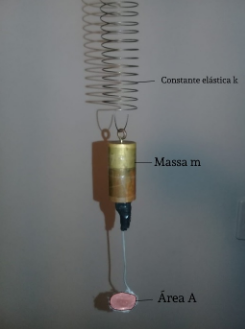
\includegraphics[width=5cm]{imagem_1.png}
			\caption{Objeto de massa $m$ e mola de constante elástica $k$ utilizados no experimento.}
			\label{fig:figura1}
		\end{figure}
	
		A determinação da massa $m$ do objeto foi feita com o auxílio de uma balança digital, cuja precisão é de $0,0001 kg$.

		\begin{figure}[H]
			\centering
			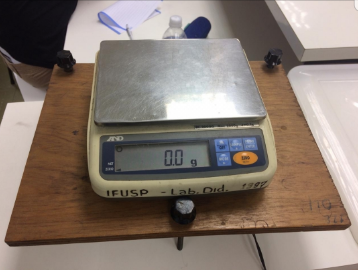
\includegraphics[width=5cm]{imagem_2.png}
			\caption{Balança digital utilizada nas diversas medições das massas relevantes ao experimento.}
			\label{fig:figura2}
		\end{figure}		
		
		Para determinar o valor da constante elástica $k$ da mola, foram analisadas as deformações às quais ela se sujeitou para que a força elástica entrasse em equilíbrio com a força peso proporcionada pela adição de massas de valores conhecidos a uma de suas extremidades. Foi montada uma tabela, contendo os valores das massas utilizadas, as forças peso correspondentes e as deformações da mola. A medição das massas foi novamente feita com o auxílio da balança digital, com resolução de $0,0001 kg$, e as medidas das deformações foram feitas com uma escala graduada, com resolução de $0,001 m$.
				
		Com os dados da tabela, foi construído um gráfico relacionando a força peso com a deformação da mola, com o auxílio do aplicativo webROOT. O coeficiente angular da reta ajustada fornece o valor da constante elástica procurada, já com uma incerteza associada às precisões dos equipamentos citados.
		
		A área $A$ da extremidade submersa do objeto foi determinada considerando que se trata de uma área circular, de raio $r$, medido com a escala graduada cuja resolução é de $0,001 m$. Assim, considerou-se válida a relação $A=\pi r^2$.
		
		\begin{figure}[H]
			\centering
			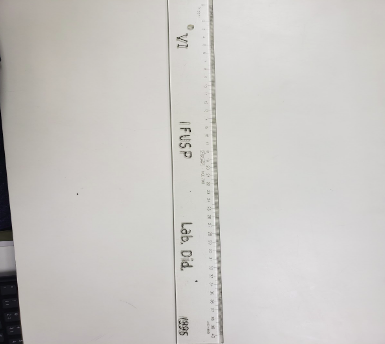
\includegraphics[width=5cm]{imagem_4.png}
			\caption{Escala graduada utilizada para as medições de comprimento relevantes ao experimento.}
			\label{fig:figura3}
		\end{figure}		
		
		
		O fluido utilizado foi água de torneira. A viscosidade $c$ não foi determinada experimentalmente, mas sim extraída de um documento publicado pela Universidade Presbiteriana Mackenzie \cite{mackenzie}, que cita, entre outras coisas, diversas propriedades da água. 

		Similarmente, o valor da aceleração da gravidade $g$ não foi determinado experimentalmente, mas extraído de um documento do Instituto de Física da Universidade de São Paulo \cite{iag} que estuda a relação entre a aceleração de queda e a massa de um corpo.
		
		Uma vez determinados os parâmetros citados, podemos estudar como eles se relacionam à função da posição do objeto com o tempo. O primeiro estágio da análise do movimento do objeto é determinar as forças que estão agindo sobre ele.

		A força de resistência ao movimento é a mais difícil de se analisar, uma vez que a geometria da extremidade do objeto utilizado no experimento difere da de uma esfera e, portanto, a Lei de Stokes não se aplica perfeitamente. Contudo, num trecho no livro Aerosol Science and Technology, de Parker C. Reist, há uma referência ao trabalho de Leith (1987), em que é realizado um estudo sobre o arrasto em objetos não-esféricos.

		Neste trabalho \cite{parker}, Leith conclui que o arrasto, nesses casos, está associado com a área de superfície do objeto, de acordo com a expressão $F_{rm}=-300\pi c (\frac{1}{3}d_p+\frac{2}{3}d_s)v$, ajustadas para unidades do SI, onde $c$ é a viscosidade do fluido, $v$ a velocidade do objeto, $d_n$ o diâmetro de uma esfera cuja área projetada é a mesma da área $A$ do objeto e $d_s$ o diâmetro de uma esfera cuja superfície efetiva é a mesma do objeto.
		
		A área projetada de uma esfera é dada por $Ap=\frac{\pi}{4}d_p^2$, e a superfície efetiva de uma esfera é dada por $A_s=\pi d_s^2 \approx 2A$.
		
		Por conveniência, o fator $300\pi c(\frac{1}{3}d_p+\frac{2}{3}d_s)$ que multiplica a velocidade da esfera será abreviado por $b$, tal que $F_{rm}= -bv$.
		
		As demais forças relevantes agindo sobre o objeto são a força peso $F_p=mg$ e a força elástica $F_e= -ky$. Portanto, a força resultante é será dada por $R=F_p+F_{rm}+F_e$. Desenvolvendo a igualdade, obtém-se a equação diferencial que descreve o movimento do objeto:
		
		\begin{align} 
			F_r &= m\frac{d^2y}{dt^2} \label{eq:equacao_1} \\
			F_r &= -ky -\rho\frac{dy}{dt} + mg \label{eq:equacao_2}
		\end{align}
		
		Fazendo a \autoref{eq:equacao_1} igual a \autoref{eq:equacao_2}
		\begin{align}
			m\frac{d^2y}{dt^2} &= -ky -\rho\frac{dy}{dt} + mg\nonumber \\
			\frac{d^2y}{dt^2} &= -\frac{k}{m}y -\frac{\rho}{m}\frac{dy}{dt} + \frac{m}{m}g \nonumber \\
			\frac{d^2y}{dt^2} &= -\frac{k}{m}y -\frac{\rho}{m}\frac{dy}{dt} + g \label{eq:equacao_3}
		\end{align}
		
		Por definição:
		\begin{align}
			\omega_0^2 \equiv \frac{k}{m} \label{eq:equacao_4}\\
			\gamma \equiv \frac{\rho}{m} \label{eq:equacao_5}			
		\end{align}
		
		Substituindo a \autoref{eq:equacao_4} e \autoref{eq:equacao_5} na \autoref{eq:equacao_3}
		\begin{align}
			\frac{d^2y}{dt^2} &=-\omega_0^2y -\gamma\frac{dy}{dt} + g\nonumber \\
			\frac{d^2y}{dt^2}+\gamma\frac{dy}{dt}+\omega_0^2y &=g \label{eq:equacao_6}
		\end{align}
		
		Através da solução complexa na \autoref{eq:equacao_7}:
		\begin{align}
			z(t) &= y(t) + i x(t) \label{eq:equacao_7} 
		\end{align}
		
		\begin{align}
			\frac{d^2y}{dt^2}+\gamma\frac{dy}{dt}+\omega_0^2y &=g \cos(\omega t) \label{eq:equacao_8} \\
			i\biggl(\frac{d^2x}{dt^2}+\gamma\frac{dx}{dt}+\omega_0^2x\biggr) &=ig\sin(\omega t) \label{eq:equacao_9}
		\end{align}
		
		Somando a \autoref{eq:equacao_8} com a \autoref{eq:equacao_9}
		\begin{align}
			\frac{d^2(y+ix)}{dt^2}+\gamma\frac{d(y+ix)}{dt}+\omega_0^2(y+ix) &=g (\cos(\omega t)+i\sin(\omega t)) \nonumber \\
			\frac{d^2z}{dt^2}+\gamma\frac{dz}{dt}+\omega_0^2z &=ge^{i\omega t} \label{eq:equacao_10}
		\end{align}
		
		Sendo:
		\begin{align}
			z(t) = Z_0e^{i\omega t} \label{eq:equacao_11} \\
			Z_0 = A_0e^{i\theta} \label{eq:equacao_12}
		\end{align}
		
		Tomando a primeira e a segunda derivadas da \autoref{eq:equacao_11}:
		\begin{align}
			\frac{dz}{dt} = i\omega Z_0e^{i\omega t} \Longrightarrow \frac{dz}{dt} = i\omega z(t) \label{eq:equacao_13} \\
			\frac{d^2z}{dt^2} = i^2\omega^2 Z_0e^{i\omega t} \Longrightarrow \frac{d^2z}{dt^2} = -\omega^2 z(t) \label{eq:equacao_14}
		\end{align}
		
		Substituindo a \autoref{eq:equacao_13} e a \autoref{eq:equacao_14} na \autoref{eq:equacao_10}
		\begin{align}
			-\omega^2z + i\gamma \omega z + \omega_0^2 z &= ge^{i\omega t} \nonumber \\
			z(-\omega^2 + i\gamma \omega + \omega_0^2) &= ge^{i\omega t} \nonumber \\
			z(\omega_0^2-\omega^2 + i\gamma \omega) &= ge^{i\omega t} \label{eq:equacao_15}
		\end{align}
		
		Substituindo o segundo membro da \autoref{eq:equacao_12} na \autoref{eq:equacao_15}
		\begin{align}
			Z_0e^{i\omega t}(\omega_0^2-\omega^2 + i\gamma \omega) &= ge^{i\omega t} \nonumber \\
			Z_0(\omega_0^2-\omega^2 + i\gamma \omega) &= g \label{eq:equacao_16}
		\end{align}
		
		Substituindo o segundo membro da \autoref{eq:equacao_12} na \autoref{eq:equacao_16}		
		\begin{align}
			A_0e^{i\theta}(\omega_0^2-\omega^2 + i\gamma \omega) &= g \nonumber \\
			A_0(\cos(\omega t)+i\sin(\omega t)) &= \frac{g}{\omega_0^2-\omega^2 + i\gamma \omega} \label{eq:equacao_17}
		\end{align}
		
		Multiplicando pelo conjugado do denominador da \autoref{eq:equacao_17}
		\begin{align}
			A_0(\cos(\omega t)+i\sin(\omega t)) &= \frac{g}{(\omega_0^2-\omega^2 + i\gamma \omega)} \frac{(\omega_0^2-\omega^2 - i\gamma \omega)}{(\omega_0^2-\omega^2 - i\gamma \omega)} \nonumber \\
			A_0(\cos(\omega t)+i\sin(\omega t)) &= \frac{g(\omega_0^2-\omega^2 - i\gamma \omega)}{(\omega_0^2-\omega^2)^2+\gamma^2 \omega^2} \label{eq:equacao_18}
		\end{align}
		
		Tomando a parte Real da \autoref{eq:equacao_18} e a parte Imaginaria da \autoref{eq:equacao_18}:
		\begin{align}
			A_0\cos(\theta) &= \frac{g(\omega_0^2-\omega^2)}{[(\omega_0^2-\omega^2)^2+\gamma^2 \omega^2]}  \label{eq:equacao_19}\\
			A_0\sin(\theta) &= \frac{g\gamma \omega}{[(\omega_0^2-\omega^2)^2+\gamma^2 \omega^2]} \label{eq:equacao_20}
		\end{align}
		
		Somando o quadrado da \autoref{eq:equacao_19} e o quadrado da \autoref{eq:equacao_20}
		\begin{align}
			A_0^2\cos^2(\theta) &= \frac{g^2(\omega_0^2-\omega^2)^2}{[(\omega_0^2-\omega^2)^2+\gamma^2 \omega^2]^2} \nonumber \\
			A_0^2\sin^2(\theta) &= \frac{g^2\gamma^2 \omega^2}{[(\omega_0^2-\omega^2)^2+\gamma^2 \omega^2]^2} \nonumber \\
			A_0^2(\cos^2(\theta) + \sin^2(\theta)) &= \frac{g^2(\omega_0^2-\omega^2)^2}{[(\omega_0^2-\omega^2)^2+\gamma^2 \omega^2]^2}+\frac{g^2\gamma^2 \omega^2}{[(\omega_0^2-\omega^2)^2+\gamma^2 \omega^2]} \nonumber \\
			A_0^2 &= \frac{g^2(\omega_0^2-\omega^2)^2 + g^2\gamma^2 \omega^2}{[(\omega_0^2-\omega^2)^2+\gamma^2 \omega^2]^2} \nonumber \\
			A_0^2 &= g^2\frac{(\omega_0^2-\omega^2)^2 + \gamma^2 \omega^2}{[(\omega_0^2-\omega^2)^2+\gamma^2 \omega^2]^2} \nonumber \\
			A_0 &= \frac{g}{\sqrt{(\omega_0^2-\omega^2)^2+\gamma^2 \omega^2}} \label{eq:equacao_21}
		\end{align}
		
		Sendo $g=cte$ vamos substituir o valor de $\omega = 0$ na \autoref{eq:equacao_21}:
		\begin{align}
			A_0 &= \frac{g}{\sqrt{(\omega_0^2)^2}} \nonumber \\
			A_0 &= \frac{g}{\omega_0^2} \nonumber \\
			g &= A_0\omega_0^2 \label{eq:equacao_22}
		\end{align}
		
		Substituindo \autoref{eq:equacao_22} na \autoref{eq:equacao_6}:
		\begin{align}
			\frac{d^2y}{dt^2}+\gamma\frac{dy}{dt}+\omega_0^2y &=A_0\omega_0^2 \nonumber \\
			\frac{d^2y}{dt^2}+\gamma\frac{dy}{dt}+\omega_0^2y - A_0\omega_0^2&=0 \nonumber \\
			\frac{d^2y}{dt^2}+\gamma\frac{dy}{dt}+\omega_0^2(y - A_0)&=0 \label{eq:equacao_23}
		\end{align}
		
		Definido $T(t) = y(t) - A_0$, $y(t) = T(t)+A_0$ e substituindo na \autoref{eq:equacao_23} obtemos na \autoref{eq:equacao_24} uma equação de um MHS amortecido onde ja conhecemos as suas soluções
		\begin{align}
			\frac{d^2(T+A_0)}{dt^2}+\gamma\frac{d(T+A_0)}{dt}+\omega_0^2(T)&=0 \nonumber \\
			\frac{d^2T}{dt^2}+\gamma\frac{dT}{dt}+\omega_0^2(T)&=0 \label{eq:equacao_24}
		\end{align}
		
		Soluções conhecidas do MHS Amortecido a partir da \autoref{eq:equacao_24}
		\begin{align}
			T(t)=Ae^{-\frac{\gamma}{2}t}cos(\omega t+ \varphi) \label{eq:equacao_25}
		\end{align}		
		
		Substituindo $T(t)=y(t)-A_0$ na \autoref{eq:equacao_25}:
		\begin{align}
			y(t)-A_0&=Ae^{-\frac{\gamma}{2}t}cos(\omega t+ \varphi) \nonumber \\
			y(t)&=Ae^{-\frac{\gamma}{2}t}cos(\omega t+ \varphi)+A_0 \label{eq:equacao_26}
		\end{align}
		
		onde:
		$\omega=\sqrt{\frac{k}{m}}$ 
		e
		$\gamma=\frac{b}{m}$.
		
		O procedimento experimental a ser utilizado para a coleta de dados envolve, inicialmente, acoplar a extremidade superior da mola ao suporte e a extremidade inferior no objeto.
		
		Quando o objeto estiver pendurado e em repouso, sua extremidade inferior deverá permanecer parcialmente submersa no fluido contido no recipiente, pois o atrito entre a extremidade e o fluido será responsável pelo amortecimento desejado.
		
		Ativa-se o gravador de vídeo, que deverá permanecer imóvel durante a gravação, e em seguida deforma-se a mola um pouco além da sua posição de equilíbrio com a força peso, ocasionando o início do movimento periódico do objeto.
		
		Após obtido aproximadamente um minuto de gravação, um software de análise de vídeo, Tracker, é utilizado para acompanhar a posição do objeto no decorrer do vídeo, fornecendo uma tabela de dados.
		\newpage
				
	\section*{Resultados de medições, cálculos e análise de dados}
		
		O valor obtido experimentalmente para a massa do corpo foi $m=0,1007\pm0,0001 kg$.
		
		A tabela abaixo contém os dados relevantes para o cálculo da constante elástica $k$ da mola.
		
		\begin{table}[H]
			\centering
			\begin{tabular}{|l|l|l|}
				\hline
				Massa $(kg) \pm 0,0001$ & Peso $(N) \pm 0,001$ & Deformação $(m) \pm 0,001$ \\ \hline
				0,0502              & 0,491             & 0,056                 \\ \hline
				0,0213              & 0,208             & 0,017                 \\ \hline
				0,0401              & 0,392             & 0,043                 \\ \hline
				0,0316              & 0,309             & 0,034                 \\ \hline
				0,0615              & 0,602             & 0,074                 \\ \hline
			\end{tabular}
			\caption{Dados obtidos para a determinação da constante elástica da mola
			}
			\label{tab:table1}
		\end{table}
		
		\begin{figure}[H]
			\centering
			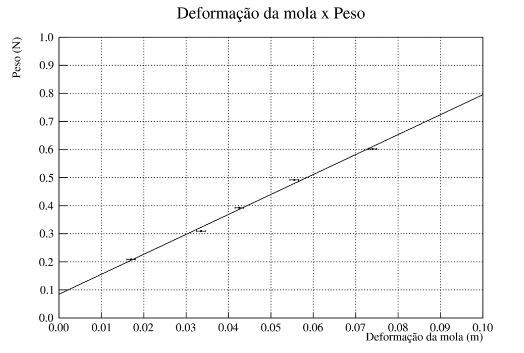
\includegraphics[width=15cm]{grafico_1.png}
			\caption{Gráfico do peso em função da deformação da mola.}
			\label{graf:grafico1}
		\end{figure}
		
		De acordo com o aplicativo webROOT, o coeficiente angular da reta ajustada, e portanto, o valor da constante elástica da mola é $k=7,10 \pm 0,17 \frac{N}{m}$.
		
		O valor obtido experimentalmente para o raio da extremidade do objeto foi $r=0,0095 \pm 0,001 m$. Portanto, a área da extremidade é $A=\pi 0,0095^2 = 0,0002835 m^2$, com incerteza $\sigma_A$ dada por:
		
		\begin{align}
			\sigma_A &= \frac{\partial A}{\partial r}.\sigma_r \nonumber \\
			\sigma_A &= 2.\pi.r.\sigma_r \nonumber \\
			\sigma_A &= 2.\pi.0,0095.0,001 \nonumber \\
			\sigma_A &= 0,0000597 m^2 \nonumber
		\end{align}
		
		As constantes extraídas de outros documentos foram a viscosidade da água e a aceleração da gravidade, cujos respectivos valores são $c=0,0008903 Pas$ e $g=9,7864 ms^{-2}$.
	
		Resta agora calcular o fator $b$, presente na força de resistência $F_{rm}$, e para isso, é necessário calcular os diâmetros $d_p$ e $d_s$, além de suas respectivas incertezas.
		
		\begin{align}
			d_p = \sqrt{\frac{4A}{\pi}} \Rightarrow d_p = \sqrt{\frac{0,001134}{\pi}} \Rightarrow d_p = 0,0190 m  \nonumber \\
			\sigma_{d_p} = \frac{\partial d_p}{\partial A}\sigma_A \Rightarrow \sigma_{d_p} = \frac{\sigma_A}{\sqrt{\pi A}} \Rightarrow \sigma_{d_p} = \frac{0,0000597}{\sqrt{\pi 0,0002835}} \Rightarrow \sigma_{d_p} = 0,0020 m \nonumber \\
			d_s = \sqrt{\frac{2A}{\pi}} \Rightarrow d_s = \sqrt{\frac{0,000567}{\pi}} \Rightarrow d_s = 0,0134 m  \nonumber \\
			\sigma_{d_s} = \frac{\partial d_s}{\partial A}\sigma_A \Rightarrow \sigma_{d_s} = \frac{\sigma_A}{\sqrt{2\pi A}} \Rightarrow \sigma_{d_s} = \frac{0,0000597}{\sqrt{\pi 0,000567}} \Rightarrow \sigma_{d_s} = 0,0014 m \nonumber
		\end{align}
	
		Assim, o fator $b$ é dado por:
	
		\begin{align}
			b=300\pi c \biggr(\frac{1}{3}d_p+\frac{2}{3}d_s\biggl) \Rightarrow b=300\pi 0,0008903\biggr(\frac{1}{3}0,019+\frac{2}{3}0,0134\biggl) \Rightarrow  b=0,01281 kgs^-1 \nonumber
		\end{align}
		
		com incerteza $\sigma_b$ dada por:
		
		\begin{align}
			\sigma_b^2&=\biggr(\frac{\partial b}{\partial d_p} \sigma_{d_p}\biggl)^2+\biggr(\frac{\partial \sigma b}{\partial d_s} \sigma_{d_s}\biggl)^2 \nonumber \\
			\sigma_b^2&=(100\pi \times 0,0008903 \times 0,002)^2+(2\times 100\pi\times 0,0008903\times 0,0014)^2 \nonumber \\
			\sigma_b &=\sqrt{0,0000009262} \nonumber \\
			\sigma_b &= 0,00096 kgs^-1. \nonumber
		\end{align}
	
		\newpage	
		A tabela à seguir exibe todos os dados relevantes obtidos nesta etapa do procedimento experimental.
		\begin{table}[H]
			\centering
			\begin{tabular}{|l|l|}
				\hline
				Massa do objeto $(kg) \pm 0,0001$ & 0,1007 \\ \hline
				Constante elástica da mola $(\frac{N}{m}) \pm 0,2$ & 7,1 \\ \hline
				Área da extremidade $(m^2) \pm 0,00006$ & 0,00028 \\ \hline
				Viscosidade da água $(Pa\times s)$ & 0,0009 \\ \hline
				Aceleração da gravidade $(\frac{m}{s^2})$ & 9,79 \\ \hline
			\end{tabular}
			\caption{Dados relevantes para o estudo do movimento do objeto
			}
			\label{tab:table2}
		\end{table}
	
		Com esses dados, é possível calcular os valores da frequência angular $\omega$ e do coeficiente de amortecimento $\gamma$, além de suas respectivas incertezas.
		
		\begin{align}
			\omega&=\sqrt{\frac{k}{m}} \nonumber \\
			\omega&=\sqrt{\frac{7,1}{0,1007}} \nonumber \\
			\omega&=8,3968 \frac{rad}{s}. \nonumber
		\end{align}
			
		\begin{align}
			\sigma_{\omega}^2 &= \biggr(\frac{\partial\omega}{\partial k}\sigma_k\biggl)^2 + \biggr(\frac{\partial\omega}{\partial m}\sigma_m\biggl)^2 \nonumber \\
			\sigma_{\omega}^2 &= \biggr(\frac{\sigma k}{2\sqrt{mk}}\biggl)^2 + \biggr(\frac{-\sqrt{k}}{2\sqrt[3]{m^2}}\sigma_m\biggl)^2 \nonumber \\
			\sigma_{\omega} &= \sqrt{\biggr(\frac{0,17}{2\sqrt{0,1007\times7,1}}\biggl)^2 + \biggr(\frac{-\sqrt{7,1}}{2\sqrt[3]{0,1007^2}}\times 0,0001\biggl)^2} \nonumber \\
			\sigma_{\omega} &= 0,1005 \frac{rad}{s} \nonumber
		\end{align}
		
		\begin{align}
			\gamma &= \frac{b}{m} \nonumber \\
			\gamma &= \frac{0,01281}{0,1007} \nonumber \\
			\gamma &= 0,1273 s^{-1} \nonumber
		\end{align}
		
		\begin{align}
			\sigma_{\gamma}^2 &= \biggr(\frac{\partial\gamma}{\partial b}\sigma_b\biggl)^2 + \biggr(\frac{\partial\gamma}{\partial m}\sigma_m\biggl)^2 \nonumber \\
			\sigma_{\gamma}^2 &= \biggr(\frac{\sigma_b}{m}\biggl)^2 + \biggr(\frac{-b\sigma_m}{m^2}\biggl)^2 \nonumber \\
			\sigma_\gamma &= \sqrt{\biggr(\frac{0,00096}{0,1007}\biggl)^2 + \biggr(\frac{-0,01281\times 0,0001}{0,1007^2}\biggl)^2} \nonumber \\
			\sigma_\gamma &= 0,0095 s^{-1} \nonumber
		\end{align}
		
		Assim, os valores esperados para o coeficiente de amortecimento e para a frequência angular, considerando o aparato instrumental utilizado, estão na tabela abaixo.
		\begin{table}[H]
			\centering
			\begin{tabular}{|l|l|}
				\hline
				Frequência angular $(\frac{rad}{s}) \pm 0,1$ & Coeficiente de amortecimento $(\frac{1}{s}) \pm 0,01$ \\ \hline
				8,4              & 0,13 \\ \hline
			\end{tabular}
			\caption{Dados obtidos para a determinação da constante elástica da mola
			}
			\label{tab:table1}
		\end{table}		
		
		Após a realização do experimento, de acordo com o procedimento experimental indicado, o aplicativo Tracker forneceu uma tabela, indicando a posição do objeto em cada frame registrado pelo gravador. Como foram registrados ao todo quase dois mil valores pelo aplicativo, os valores serão apresentados graficamente.
		
		\begin{figure}[H]
			\centering
			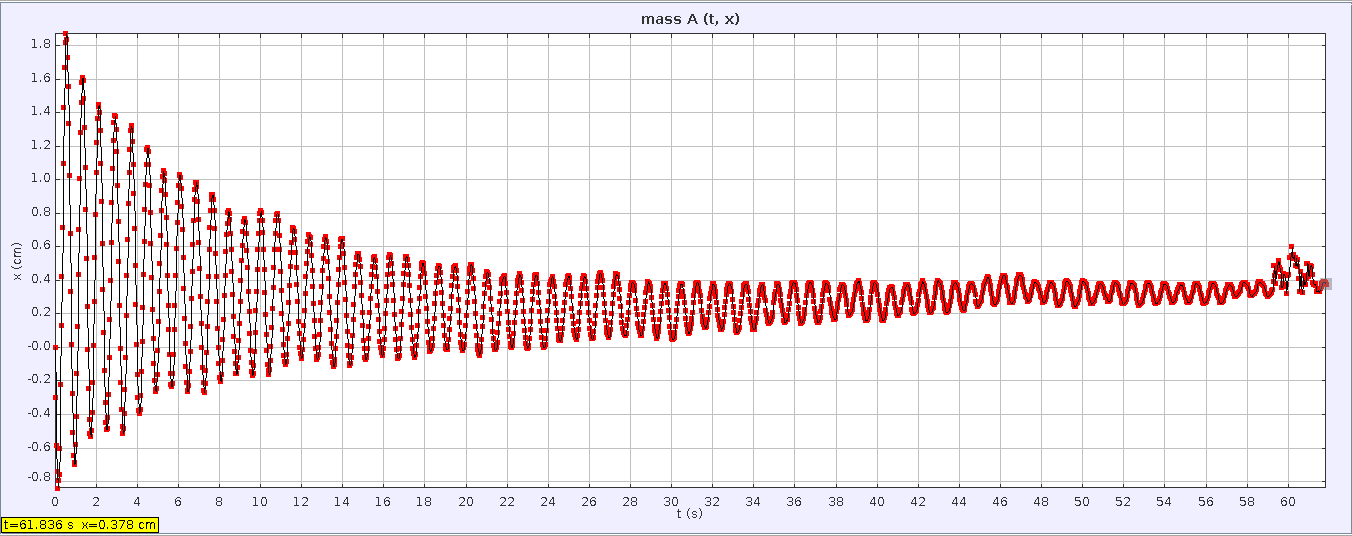
\includegraphics[width=13cm]{figura_3.png}
			\caption{Dados referentes à posição do objeto em função do tempo, obtidos através do aplicativo Tracker.}
			\label{fig:figura3}
		\end{figure}
	
		Considerando apenas os dados no intervalo $6\leq t \leq 22 s$, foi montado novamente um gráfico, dessa vez no aplicativo webROOT, a fim de obter os valores dos parâmetros experimentais através do ajuste da curva. Os dados considerados e o ajuste obtido constam nos gráficos a seguir.

		\begin{figure}[H]
			\centering
			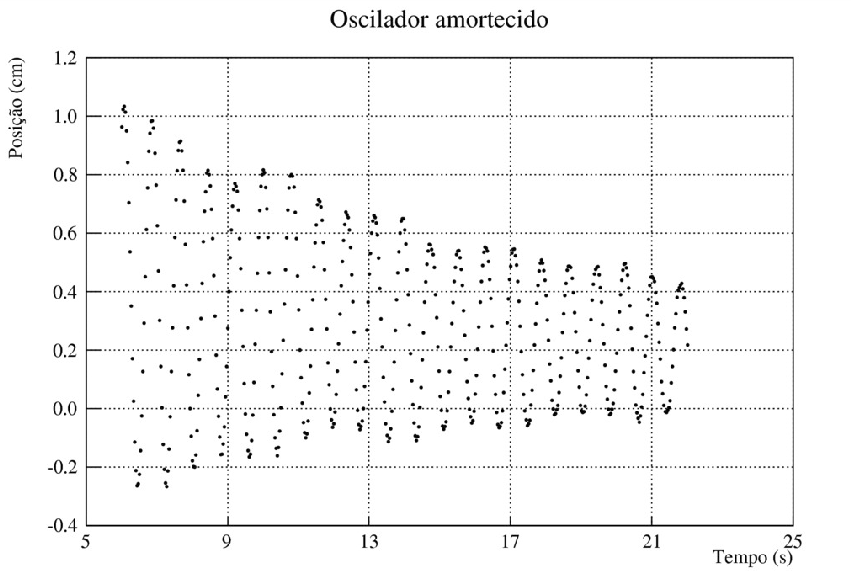
\includegraphics[width=13cm]{grafico_4.png}
			\caption{ Dados considerados para a obtenção dos parâmetros através do ajuste da curva.}
			\label{fig:grafico_4}
		\end{figure}	
	
		\begin{figure}[H]
			\centering
			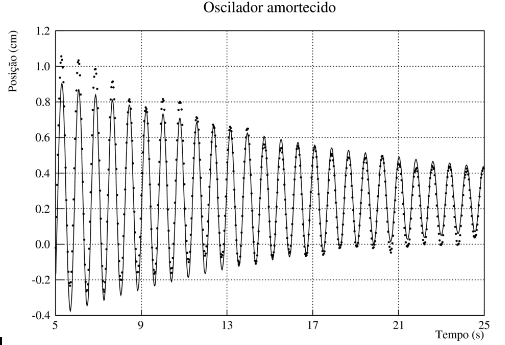
\includegraphics[width=13cm]{grafico_5.png}
			\caption{Curva obtida através do ajuste}
			\label{fig:grafico_5}
		\end{figure}
	
		Os valores obtidos para cada um dos parâmetros, com suas respectivas incertezas (calculadas pelo webROOT com base nas incertezas da posição e do instante de tempo), encontram-se na tabela à seguir.

		\begin{table}[H]
			\centering
			\begin{tabular}{|l|l|}
				\hline
				$A (cm) \pm 0,007$ & 0,913   \\ \hline
				$\omega (\frac{rad}{s}) \pm 0,001$ & 7,986 \\ \hline
				$\varphi (rad) 0,01$ &  1,71\\ \hline
				$\gamma (s^{-1}) \pm 0,001$ & 0,129 \\ \hline
				$y_0 (cm) \pm 0,001$ & 0,255 \\ \hline
			\end{tabular}
			\caption{Parâmetros obtidos através do ajuste da curva.}
			\label{tab:table2}
		\end{table}	

		Nota-se que com o ajuste da função do tipo $y(t)=Ae^{-\frac{\gamma}{2}t}\cos(\omega t + \varphi)$, que a curva obtida não contém uma boa parte dos pontos, que parecem variar em relação à curva ajustada com um comportamento oscilatório. Assim, foi considerada uma nova tentativa de ajuste, considerando uma soma de soma de seno e cosseno para descrever com maior precisão o comportamento da posição do objeto.
	
		O gráfico à seguir mostra a curva obtida através do ajuste com uma função do tipo $y(t)=Ae^{-\frac{\gamma}{2}t}[\cos(\omega_1 t + \varphi_1)+\sin(\omega_2 t + \varphi_2)]+y_0$.
		
		\begin{figure}[H]
			\centering
			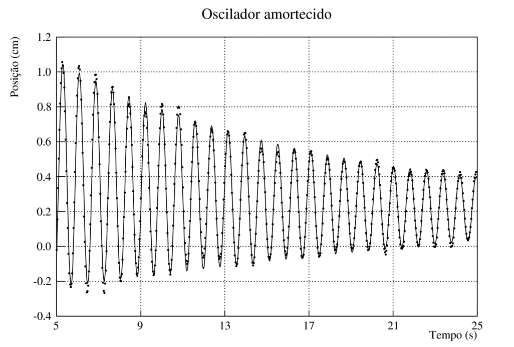
\includegraphics[width=13cm]{grafico_6.png}
			\caption{Curva obtida através do ajuste citado}
			\label{fig:grafico_6}
		\end{figure}
	
		Os valores dos parâmetros, assim como suas respectivas incertezas, estão apresentados na tabela à seguir.
		
		\begin{table}[H]
			\centering
			\begin{tabular}{|l|l|}
				\hline
				$A (cm) \pm 0,006$ & 0,893   \\ \hline
				$\omega_1 (\frac{rad}{s}) \pm 0,001$ & 7,992 \\ \hline
				$\varphi_1 (rad) 0,015$ &  1,645\\ \hline
				$\omega_2 (\frac{rad}{s})\pm 0,006$ & -0,026 \\ \hline
				$\varphi_2 (rad)\pm 0,015$ & 0,356 \\ \hline
				$\gamma (s^{-1}) \pm 0,001$ & 0,127 \\ \hline
				$y_0 (cm) \pm 0,025$ & 0,092 \\ \hline
			\end{tabular}
			\caption{Parâmetros obtidos através do ajuste da curva}
			\label{tab:table2}
		\end{table}	
	
		Alguns parâmetros, entre eles a amplitude, a fase da oscilação e a posição inicial do objeto, não dependem das características da mola ou da massa utilizada, mas apenas das condições iniciais impostas ao sistema. Por isso não foram feitas previsões para os valores de $A$, $\varphi$ ou $y_0$.
		
		Por outro lado, a frequência angular  e o coeficiente de amortecimento , como vimos nas equações  \ref{eq:equacao_4} e \ref{eq:equacao_5}, foram calculados pois dependem das características do objeto e da mola.
		
		Agora poderão ser feitas comparações entre os valores calculados teoricamente e obtidos experimentalmente. Essas comparações serão feitas através de testes-z, que estimará a correspondência dos resultados considerando suas incertezas. A expressão utilizada para comparação de resultados  através do teste-z é: $z=\frac{\bar a - \bar b}{\sqrt{\sigma_a^2+\sigma_b^2}}$. A tabela à seguir contém os valores a serem comparados e suas respectivas incertezas.

		\begin{table}[H]
			\centering
			\begin{tabular}{|l|l|}
				\hline
				Frequência ângular teórica $\omega_T (\frac{rad}{s})$ & $8,4 \pm 0,1$   \\ \hline
				Frequência angular experimental do primeiro ajuste $\omega_{E_1} (\frac{rad}{s})$ & $7,986 \pm 0,001$ \\ \hline
				Frequência angular experimental do segundo ajuste $\omega_{E_2} (\frac{rad}{s})$ & $7,992 \pm 0,001$ \\ \hline
				Coeficiente de amortecimento teórico $\gamma_T (\frac{1}{s})$ & $0,13\pm0,01$ \\ \hline
				Coeficiente de amortecimento experimental do primeiro ajuste $\gamma_{E_1} (\frac{1}{s})$ & $0,129\pm0,001$ \\ \hline
				Coeficiente de amortecimento experimental do segundo ajuste $\gamma_{E_2} (\frac{1}{s})$ & $0,127\pm0,001$ \\ \hline
			\end{tabular}
			\caption{Parâmetros obtidos através do ajuste da curva}
			\label{tab:table2}
		\end{table}
	
		O teste-z entre a frequência angular teórica e a frequência angular experimental do primeiro ajuste é dado por:
		
		\begin{align}
			Z_1 &= \frac{\omega_T - \omega_{E_1}}{\sqrt{\sigma_{\omega_T}^2+\sigma_{\omega_{E_1}}^2}} \nonumber \\
			Z_1 &= \frac{8,4 - 7,986}{\sqrt{0,1^2+0,001^2}} \nonumber \\
			Z_1 &= 4,14 \nonumber
		\end{align}
		
		Similarmente, o teste-z entre a frequência angular teórica e a frequência angular experimental do segundo ajuste é dado por:
		
		\begin{align}
			Z_2 &= \frac{\omega_T - \omega_{E_2}}{\sqrt{\sigma_{\omega_T}^2+\sigma_{\omega_{E_2}}^2}} \nonumber \\
			Z_2 &= \frac{8,4 - 7,992}{\sqrt{0,1^2+0,001^2}} \nonumber \\
			Z_2 &= 4,08 \nonumber
		\end{align}
		
		O teste-z entre o coeficiente de amortecimento teórico e o coeficiente de amortecimento experimental do primeiro ajuste é dado por:

		\begin{align}
			Z_3 &= \frac{\gamma_T - \gamma_{E_1}}{\sqrt{\sigma_{\gamma_T}^2+\sigma_{\gamma_{E_1}}^2}} \nonumber \\
			Z_3 &= \frac{0,13 - 0,129}{\sqrt{0,1^2+0,001^2}} \nonumber \\
			Z_3 &= 0,1 \nonumber
		\end{align}		
		
		E, finalmente, o teste-z entre o coeficiente de amortecimento teórico e o coeficiente de amortecimento experimental do primeiro ajuste é dado por:
		\begin{align}
			Z_4 &= \frac{\gamma_T - \gamma_{E_2}}{\sqrt{\sigma_{\gamma_T}^2+\sigma_{\gamma_{E_2}}^2}} \nonumber \\
			Z_4 &= \frac{0,13 - 0,127}{\sqrt{0,1^2+0,001^2}} \nonumber \\
			Z_4 &= 0,3 \nonumber
		\end{align}
		
		Observando os resultados dos testes realizados, nota-se que as compatibilidades das frequências angulares experimentais com a teórica foram bem próximas de $4\sigma$, enquanto as compatibilidades dos coeficientes de amortecimento experimentais com o teórico foram ambos menores que $1\sigma$.
		
		Assim, os resultados referentes ao coeficiente de amortecimento foram muito satisfatórios, enquanto os resultados referentes à frequência angular foram razoavelmente satisfatórios (não tiveram compatibilidade de até $3\sigma$, mas entre $3\sigma$ e $5\sigma$).
		
		Essa divergência na frequência angular provavelmente está associada com alguns fatores não levados em consideração. Foram desconsideradas as pequenas oscilações do corpo em outras direções que não a vertical, assim como a massa da mola nos cálculos efetuados, entre outros detalhes que aparentemente culminaram na divergência observada. Essa é apenas uma hipótese, no entanto, e testar sua validade envolveria novas etapas para o experimento.
		
							
	
	\section*{Discussão final e conclusões}
		A estratégia utilizada para a coleta de dados foi adequada, uma vez que, com os dados obtidos experimentalmente, foi possível determinar um ajuste na forma de uma equação diferencial de segunda ordem e de coeficientes constantes para descrever a posição do objeto. 
		
		As equações e constantes extraídas de outros documentos e utilizadas para a especulação dos valores teóricos foram muito precisas. No entanto, nem todos os valores obtidos através do ajuste para os parâmetros relacionados à posição do objeto foram exatos.
		
		Em particular, a frequência angular obtida experimentalmente divergiu ligeiramente daquela obtida teoricamente, provavelmente em função do descarte de alguns fatores inicialmente julgados menos relevantes, como as oscilações horizontais e longitudinais do objeto e as perdas de energia da mola. De modo geral, o experimento foi bem sucedido e os resultados obtidos foram satisfatórios.

	\newpage
	
	\begin{thebibliography}{99}
		\bibitem{parker} Parker C. Reist
		\emph{Aerosol Science and Technology}.
		Addison-Wesley (1986).
		
		\bibitem{moyses} Moysés Nussenzveig
		\emph{Curso de Física Básica Vol. 2}.
		Blucher (2014).

		\bibitem{mackenzie} 
		Algumas propriedades de Fluidos - Universidade Mackenzie, Acessado em (02/12/2019)
		\\\texttt{http://meusite.mackenzie.com.br/miriamtg/portfolio\_FT\_I/portfolio\_FT\_I\_ap\_E.pdf}
			
		\bibitem{iag} 
		Determinação da aceleração gravitacional - IAG-USP, Acessado em (02/12/2019)
		\\\texttt{http://www2.if.usp.br/\~eletivos/posters\_2005/painel13.pdf}
		
	\end{thebibliography}

\end{document}